\section{Results}
\label{sec:experiments}

We report results on the 960 matched FULL/Sharded pairs (\cref{sec:stats}), organized around three research questions: whether models lose track of constraints under sharding (\cref{sec:rq1}), whether the five creative-quality dimensions shift under sharding (\cref{sec:rq2}), and whether any quality shift survives once instruction adherence is held equal between the two conditions (\cref{sec:rq3}). \cref{fig:main_results} previews all three: FULL improves constraint adherence and structure/coherence with the largest standardized effects; craft's overall improvement for FULL shrinks toward zero once adherence is held equal; and originality's SHARDED advantage grows at equal adherence while genre effectiveness and characterization shift toward SHARDED.

\begin{figure}[t]
\centering
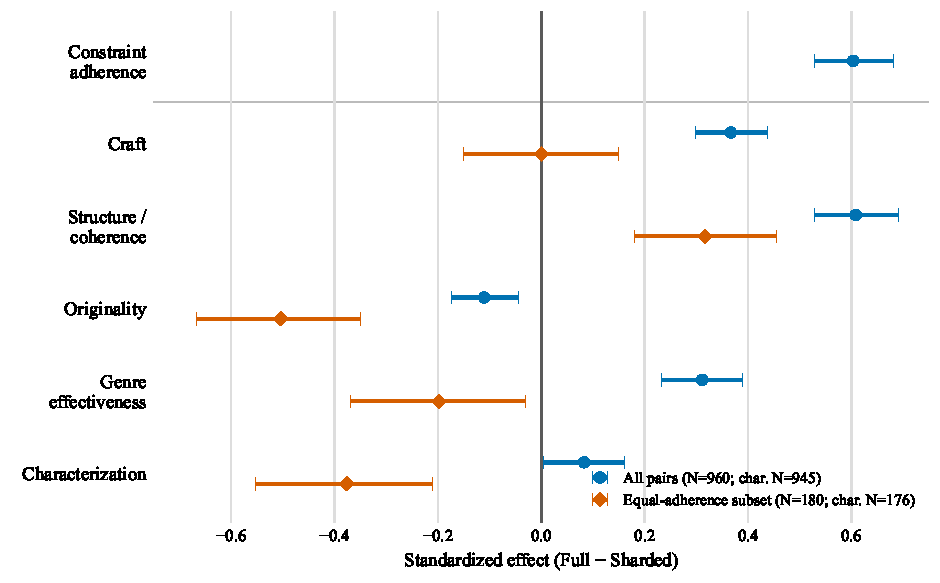
\includegraphics[width=\linewidth]{figures/figure1_main_results_forest.pdf}
\caption{Effect of prompt delivery on constraint adherence and writing-quality dimensions. Points show the standardized paired FULL$-$SHARDED effect size $d_{\mathrm{av}}$ (\cref{eq:dav}); positive values favor FULL and negative values favor SHARDED. Error bars denote 95\% story-clustered bootstrap confidence intervals (\cref{sec:stats}). Circles show all 960 matched model--task pairs, while diamonds show the subset of pairs with equal constraint-adherence scores (N=180; $\delta_{\mathrm{adherence}}=0$) --- omitted for constraint adherence itself, where that subset's difference is zero by construction rather than an estimate. The persistence of a positive structure/coherence effect in the equal-adherence subset suggests that the structural degradation associated with multi-turn specification is not explained solely by constraint loss. Writing-quality dimensions are automated rubric-based judgments rather than direct measures of human creative preference.}
\label{fig:main_results}
\end{figure}

\begin{table}[t]
\centering
\small
\begin{tabular}{lrrrrl}
\toprule
\textbf{Dimension} & \textbf{N} & \textbf{FULL} & \textbf{SHARDED} & \textbf{$\delta$ (FULL$-$SHARDED)} & \textbf{95\% CI} \\
\midrule
Constraint adherence & 960 & 0.852 & 0.742 & $+$0.111 & [0.096, 0.126] \\
Craft                & 960 & 3.044 & 2.796 & $+$0.248 & [0.200, 0.295] \\
Structure/coherence  & 960 & 3.231 & 2.755 & $+$0.476 & [0.413, 0.542] \\
Originality          & 960 & 2.447 & 2.525 & $-$0.078 & [$-$0.123, $-$0.032] \\
Genre effectiveness  & 960 & 3.125 & 2.900 & $+$0.225 & [0.168, 0.280] \\
Characterization      & 945 & 2.634 & 2.580 & $+$0.054 & [0.004, 0.104] \\
\bottomrule
\end{tabular}
\caption{Raw paired FULL/SHARDED means, the raw paired difference $\delta$ (\cref{eq:delta}), and its 95\% story-clustered bootstrap confidence interval, over all matched pairs (constraint adherence is on a 0--1 scale; the five quality dimensions are on a 1--5 scale). Characterization is scored for fewer pairs because it is left null for items with no character-driven requirement (\cref{sec:constraints}).}
\label{tab:main_results}
\end{table}

\subsection{RQ1: Constraint Adherence}
\label{sec:rq1}

FULL substantially improves constraint adherence over Sharded. Mean adherence is 0.852 under FULL versus 0.742 under Sharded, a raw paired difference of $+$0.111 (95\% CI [0.096, 0.126]; \cref{tab:main_results}), corresponding to one of the two largest standardized effects in the benchmark, $d_{\mathrm{av}} = 0.60$ (\cref{fig:main_results}). The interval excludes zero by a wide margin: models are consistently more likely to satisfy a story's atomic constraints when the full instruction is given upfront than when the same instruction is delivered one shard at a time.

\subsection{RQ2: Writing-Quality Dimensions}
\label{sec:rq2}

FULL also improves three of the five creative-quality dimensions. Structure/coherence shows the largest quality-dimension gap ($\delta = +0.476$, 95\% CI [0.413, 0.542], $d_{\mathrm{av}} = 0.61$), followed by craft ($\delta = +0.248$, 95\% CI [0.200, 0.295], $d_{\mathrm{av}} = 0.37$) and genre effectiveness ($\delta = +0.225$, 95\% CI [0.168, 0.280], $d_{\mathrm{av}} = 0.31$); all three intervals are bounded well away from zero. Originality moves the other way: Sharded scores slightly higher than FULL on this dimension ($\delta = -0.078$, 95\% CI [$-$0.123, $-$0.032], $d_{\mathrm{av}} = -0.11$), a small but statistically clear reversal of the direction seen on every other dimension. Characterization shows the smallest FULL advantage of the five dimensions ($\delta = +0.054$, 95\% CI [0.004, 0.104]), an interval that only narrowly excludes zero.

\subsection{RQ3: Quality at Comparable Adherence}
\label{sec:rq3}

Restricting to the 180 pairs where FULL and Sharded satisfied an equal fraction of constraints ($\delta_{\text{adherence}} = 0$) changes this picture substantially. Craft's overall FULL advantage collapses to exactly zero ($\delta = 0.000$, 95\% CI [$-$0.096, 0.097], $d_{\mathrm{av}} = 0.00$), and the SHARDED advantage on originality becomes substantially larger, while genre effectiveness and characterization flip sign to favor SHARDED (originality: $\delta = -0.361$, 95\% CI [$-$0.465, $-$0.260]; genre effectiveness: $\delta = -0.133$, 95\% CI [$-$0.242, $-$0.023]; characterization: $\delta = -0.233$, 95\% CI [$-$0.335, $-$0.127]). Structure/coherence is the one dimension where a clear FULL advantage survives: $\delta = +0.239$ (95\% CI [0.135, 0.343], $d_{\mathrm{av}} = 0.32$), an interval that stays clearly above zero even at equal observed adherence. Constraint forgetting therefore does not appear sufficient to explain the entire FULL--SHARDED quality gap: the overall craft advantage disappears among pairs with equal observed adherence, while originality, genre effectiveness, and characterization shift toward SHARDED; structure/coherence, however, retains a clear positive FULL advantage.

\subsection{Model Consistency}
\label{sec:rq4}

\cref{fig:main_results} pools all six models together; \cref{fig:model_heatmap} asks whether the pooled effect on each dimension is shared broadly across models or driven by one or two of them. Constraint adherence and structure/coherence are the only two dimensions where every one of the six models shows a positive standardized effect (adherence: $d_{\mathrm{av},m}$ ranges from $+0.54$ to $+1.35$; structure/coherence: $+0.38$ to $+1.07$), so the pooled effects on those two dimensions in \cref{sec:rq1,sec:rq2} reflect a broadly shared pattern rather than an artifact of any single model. The other four dimensions are less uniform. Genre effectiveness is positive or near zero for five of six models but clearly negative for Gemma~4 12B QAT ($d_{\mathrm{av},m} = -0.37$); craft shows the same pattern ($-0.45$ for Gemma~4 12B QAT against five positive values). Gemma~4 12B QAT is also the strongest SHARDED-favoring outlier, with an originality effect of $d_{\mathrm{av},m} = -1.25$, the most negative model-dimension effect observed. Originality itself is genuinely split at the model level rather than uniformly small: GPT-OSS~20B and Gemma~4 12B QAT are clearly negative, Llama~3.1 8B Instruct and Qwen3.5~9B are close to zero, and Granite~4 H Tiny and Mistral~7B Instruct v0.3 are clearly positive, so the small pooled originality effect reported in \cref{sec:rq2} averages over models that disagree in direction rather than describing six models that individually show a small negative effect. Characterization follows a similar pattern to genre effectiveness, positive for most models but negative for Gemma~4 12B QAT and, more mildly, GPT-OSS~20B.

\begin{figure}[t]
\centering
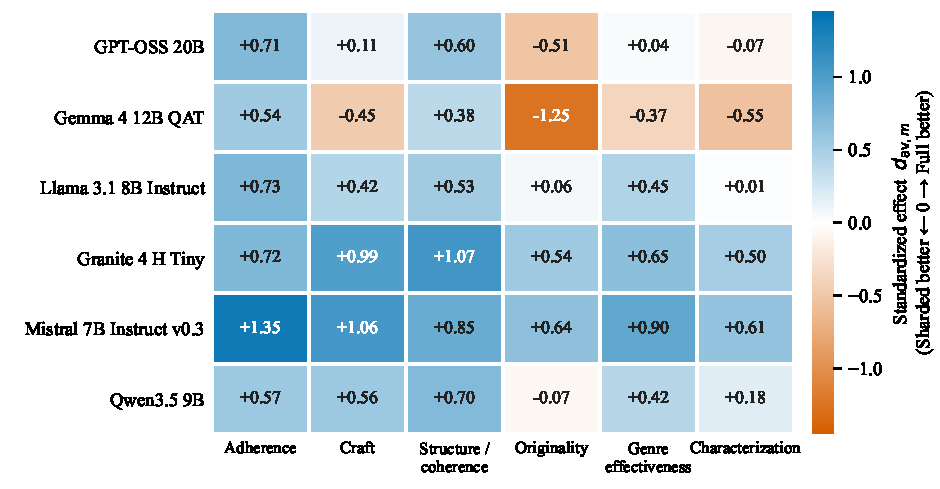
\includegraphics[width=\linewidth]{figures/figure_model_heatmap.pdf}
\caption{Model-wise standardized FULL$-$SHARDED effect $d_{\mathrm{av},m}$ (\cref{eq:dav}, computed per model over that model's 160 story pairs) for constraint adherence and each writing-quality dimension. Blue cells favor FULL, orange cells favor SHARDED, centered exactly at zero; the numeric effect is printed in every cell. No confidence intervals are shown here --- this is a point-estimate consistency check across models, not a hypothesis test (see \cref{fig:main_results} for the pooled effect with confidence intervals). Adherence and structure/coherence are positive for all six models; craft, originality, genre effectiveness, and characterization vary in sign across models, with Gemma~4 12B QAT showing the most consistently SHARDED-favoring pattern.}
\label{fig:model_heatmap}
\end{figure}
